\documentclass[tikz,border=10pt]{standalone}
\usepackage{tikz}
\usetikzlibrary{positioning,arrows.meta,shapes.geometric,patterns,decorations.pathreplacing}

\begin{document}
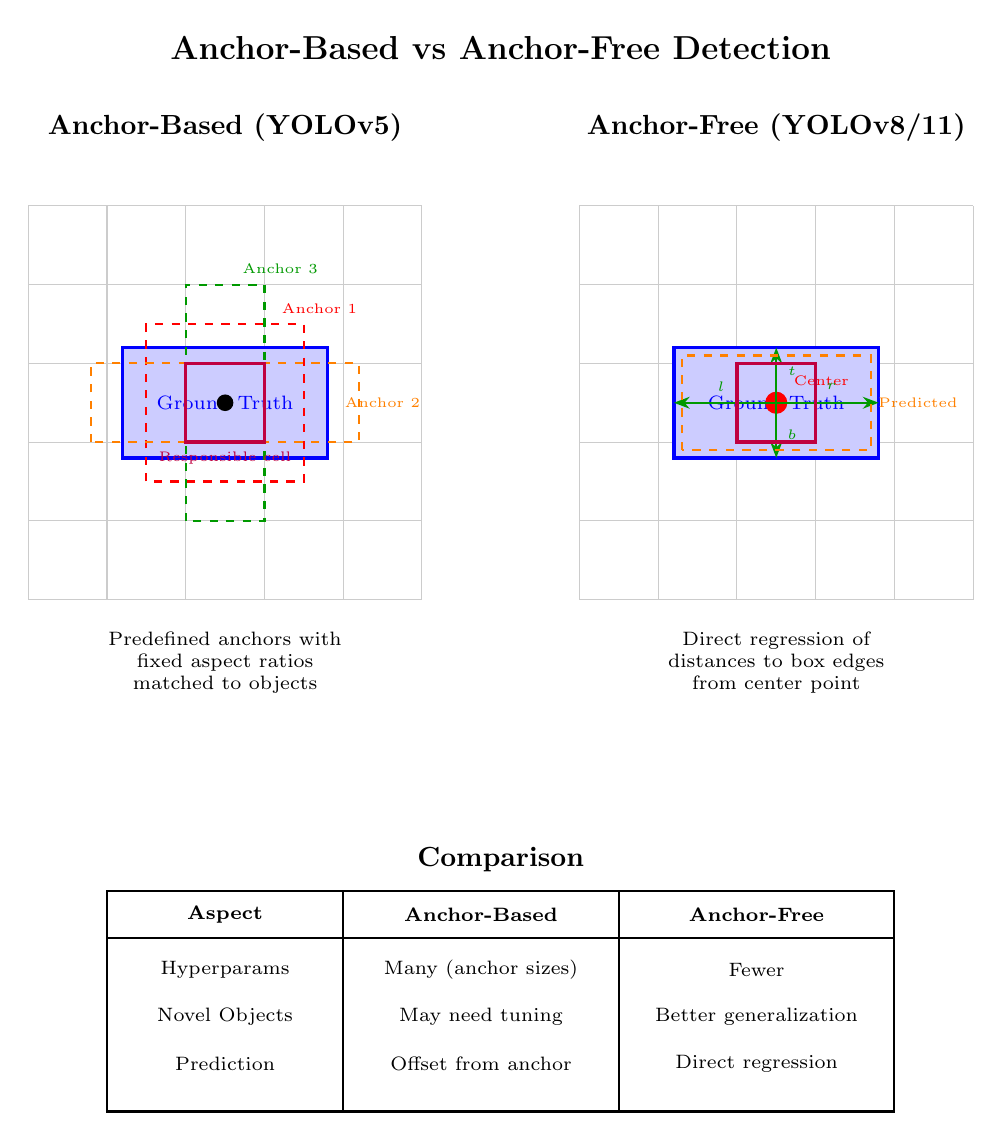
\begin{tikzpicture}[
    scale=1,
    every node/.style={font=\small}
]

% Title
\node[font=\bfseries\large] at (6,7) {Anchor-Based vs Anchor-Free Detection};

% === LEFT SIDE: Anchor-Based (YOLOv5) ===
\node[font=\bfseries] at (2.5,6) {Anchor-Based (YOLOv5)};

% Grid
\draw[step=1cm, gray!40, thin] (0,0) grid (5,5);

% Object (car-like rectangle)
\fill[blue!20] (1.2,1.8) rectangle (3.8,3.2);
\draw[blue, very thick] (1.2,1.8) rectangle (3.8,3.2);
\node[font=\scriptsize, blue] at (2.5,2.5) {Ground Truth};

% Predefined anchor boxes (different aspect ratios)
\draw[red, thick, dashed] (1.5,1.5) rectangle (3.5,3.5); % 1:1
\draw[orange, thick, dashed] (0.8,2.0) rectangle (4.2,3.0); % wide
\draw[green!60!black, thick, dashed] (2.0,1.0) rectangle (3.0,4.0); % tall

% Anchor center point
\fill[black] (2.5,2.5) circle (3pt);

% Labels for anchors
\node[font=\tiny, red] at (3.7,3.7) {Anchor 1};
\node[font=\tiny, orange] at (4.5,2.5) {Anchor 2};
\node[font=\tiny, green!60!black] at (3.2,4.2) {Anchor 3};

% Grid cell highlight
\draw[purple, very thick] (2,2) rectangle (3,3);
\node[font=\tiny, purple, below] at (2.5,2) {Responsible cell};

% Explanation text
\node[align=center, font=\scriptsize] at (2.5,-0.8) {Predefined anchors with\\fixed aspect ratios\\matched to objects};

% === RIGHT SIDE: Anchor-Free (YOLOv8) ===
\node[font=\bfseries] at (9.5,6) {Anchor-Free (YOLOv8/11)};

% Grid
\draw[step=1cm, gray!40, thin] (7,0) grid (12,5);

% Object (same car-like rectangle)
\fill[blue!20] (8.2,1.8) rectangle (10.8,3.2);
\draw[blue, very thick] (8.2,1.8) rectangle (10.8,3.2);
\node[font=\scriptsize, blue] at (9.5,2.5) {Ground Truth};

% Center point prediction
\fill[red] (9.5,2.5) circle (4pt);
\node[font=\tiny, red, above right] at (9.6,2.6) {Center};

% Direct regression arrows to box edges
\draw[-{Stealth[length=2mm]}, green!60!black, thick] (9.5,2.5) -- (8.2,2.5);
\draw[-{Stealth[length=2mm]}, green!60!black, thick] (9.5,2.5) -- (10.8,2.5);
\draw[-{Stealth[length=2mm]}, green!60!black, thick] (9.5,2.5) -- (9.5,1.8);
\draw[-{Stealth[length=2mm]}, green!60!black, thick] (9.5,2.5) -- (9.5,3.2);

% Labels for distances
\node[font=\tiny, green!60!black] at (8.8,2.7) {$l$};
\node[font=\tiny, green!60!black] at (10.2,2.7) {$r$};
\node[font=\tiny, green!60!black] at (9.7,2.1) {$b$};
\node[font=\tiny, green!60!black] at (9.7,2.9) {$t$};

% Grid cell highlight
\draw[purple, very thick] (9,2) rectangle (10,3);

% Predicted box (slightly different to show prediction)
\draw[orange, thick, dashed] (8.3,1.9) rectangle (10.7,3.1);
\node[font=\tiny, orange] at (11.3,2.5) {Predicted};

% Explanation text
\node[align=center, font=\scriptsize] at (9.5,-0.8) {Direct regression of\\distances to box edges\\from center point};

% === Bottom comparison table ===
\begin{scope}[shift={(0,-3)}]
\node[font=\bfseries] at (6,-0.3) {Comparison};

% Table
\draw[thick] (1,-0.7) rectangle (11,-3.5);
\draw[thick] (1,-1.3) -- (11,-1.3);
\draw[thick] (4,-0.7) -- (4,-3.5);
\draw[thick] (7.5,-0.7) -- (7.5,-3.5);

% Headers
\node[font=\scriptsize\bfseries] at (2.5,-1) {Aspect};
\node[font=\scriptsize\bfseries] at (5.75,-1) {Anchor-Based};
\node[font=\scriptsize\bfseries] at (9.25,-1) {Anchor-Free};

% Row 1
\node[font=\scriptsize, align=center] at (2.5,-1.7) {Hyperparams};
\node[font=\scriptsize, align=center] at (5.75,-1.7) {Many (anchor sizes)};
\node[font=\scriptsize, align=center] at (9.25,-1.7) {Fewer};

% Row 2
\node[font=\scriptsize, align=center] at (2.5,-2.3) {Novel Objects};
\node[font=\scriptsize, align=center] at (5.75,-2.3) {May need tuning};
\node[font=\scriptsize, align=center] at (9.25,-2.3) {Better generalization};

% Row 3
\node[font=\scriptsize, align=center] at (2.5,-2.9) {Prediction};
\node[font=\scriptsize, align=center] at (5.75,-2.9) {Offset from anchor};
\node[font=\scriptsize, align=center] at (9.25,-2.9) {Direct regression};

\end{scope}

\end{tikzpicture}
\end{document}
